

\section{Results} 
\label{results} 
This section summarizes the key findings of the experiments that were conducted based on the architectures presented in the sections \ref{ensemExp},  \ref{mainExperiments} and \ref{cont_learning_section} of the thesis. Additionally, this section briefly introduces the simplistic UI approach. 

\subsection{Cross-domain adaptation results}

In order to achieve fair comparison, all experiments obey the following specifications:
\begin{enumerate}
\item According to the setup defined in Figure \ref{mymodel}, the teacher model only accepts the weakly-augmented images from the \textunderscore{target} domain. Therefore, the primary objective for this ensembled model is to improve the \texttt{AP} on the teacher model. Thus, \texttt{AP50} results from the teacher model evaluation are used as the primary metric. 
\item The base learning rate is defined as \texttt{BASE\textunderscore LR} = 0.001.
\item The number of iterations is fixed as \texttt{MAX\textunderscore ITER} = 50 000.
\item The evaluation happens every \texttt{EVAL\textunderscore PERIOD} = 1000 iterations. Considering that there are 50 000 iterations total, that results in 50 evaluation points across the \texttt{AP50} plot.
\end{enumerate}  
\subsubsection{Scheduler adjustment}
\label{scheduler_section} 
First set of experiments was conducted in accordance with the \nameref{ensemExp} section. The original learning rate scheduler was used. The pattern of the original scheduler was presented earlier in Figure \ref{annealing} (a). Initially, the Adaptive teacher network was trained as it is. The results are presented in Figure \ref{original_experiment}. The first graph illustrates the evaluation \texttt{AP50} results for both the teacher and the student models. Although the training process seems idle for the first 20 000 iterations, the model eventually finds better gradients and stabilizes with $max$ (\texttt{AP50}) = 71.39\% at 31 000 iterations. Even though it might seem that the loss value is decreasing by the end of the training, the \texttt{AP50} value also steadily drops. In order to address the noisy predictions shown earlier in Figure \ref{adapt_experiment1}, the learning rate scheduler has been modified to implement a cosine annealing algorithm without restarts \cite{Loshchilov2016}, as shown in Figure \ref{annealing} (b). The original warm-up period of \texttt{WARMUP\textunderscore ITERS} = 1000 is preserved. 

\begin{figure}[htb]
	\begin{center}
		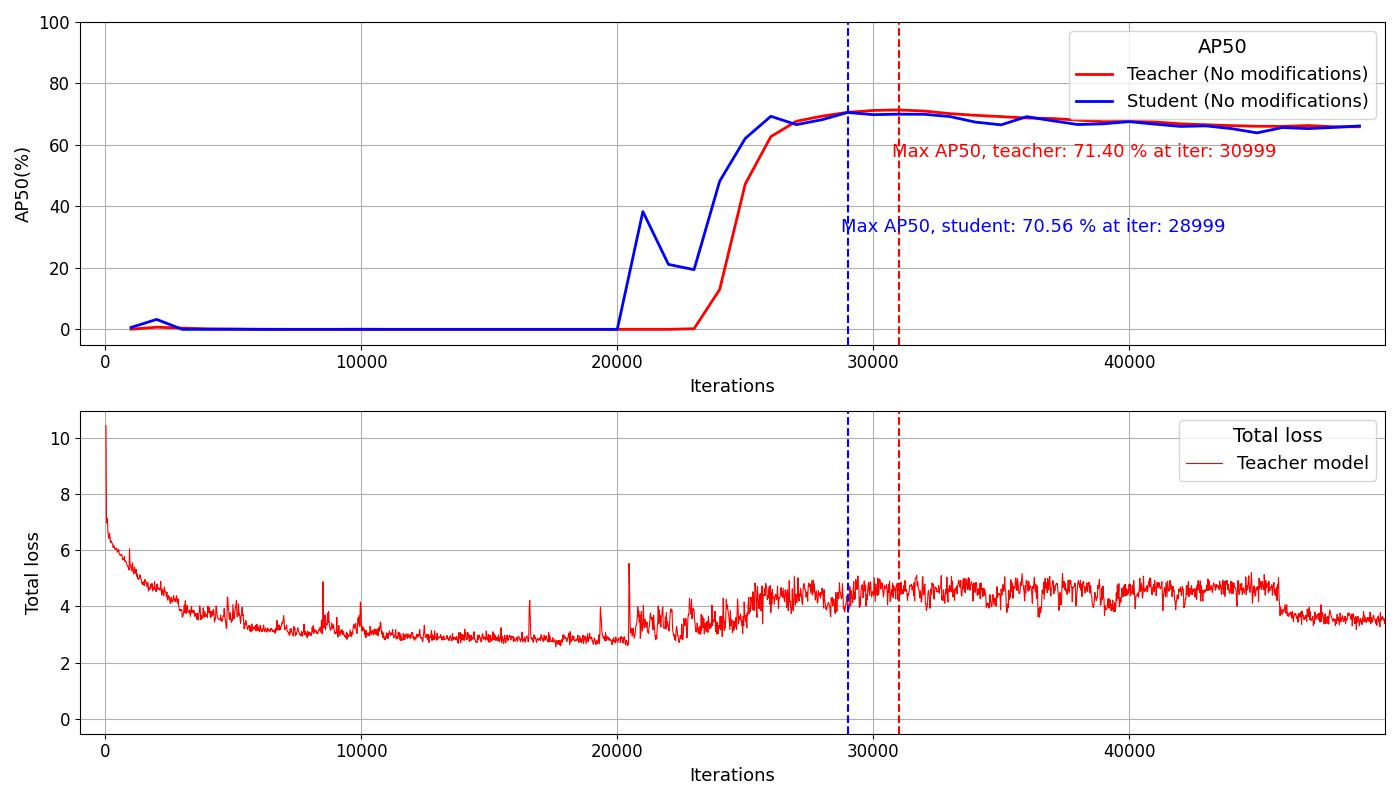
\includegraphics[width=16cm]{./loss&AP50_original.jpg}
	\end{center}
	\caption{Results of the original Adaptive teacher model evaluated on the custom T-LESS dataset without any modifications}
	\begin{center}
		\label{original_experiment}
	\end{center}
\end{figure}
\FloatBarrier
Theoretically, this setup would have allowed find better gradients and reduce overshooting. The results achieved after modifying the scheduler are shown in Figure \ref{comparison_1}. Although the \texttt{AP50} value peaked much faster with the new scheduler, it was only able to reach $max$ (\texttt{AP50}) = 62.49\%, which is almost 10\% lower than the original result.   



\begin{figure}[htb]
	\begin{center}
		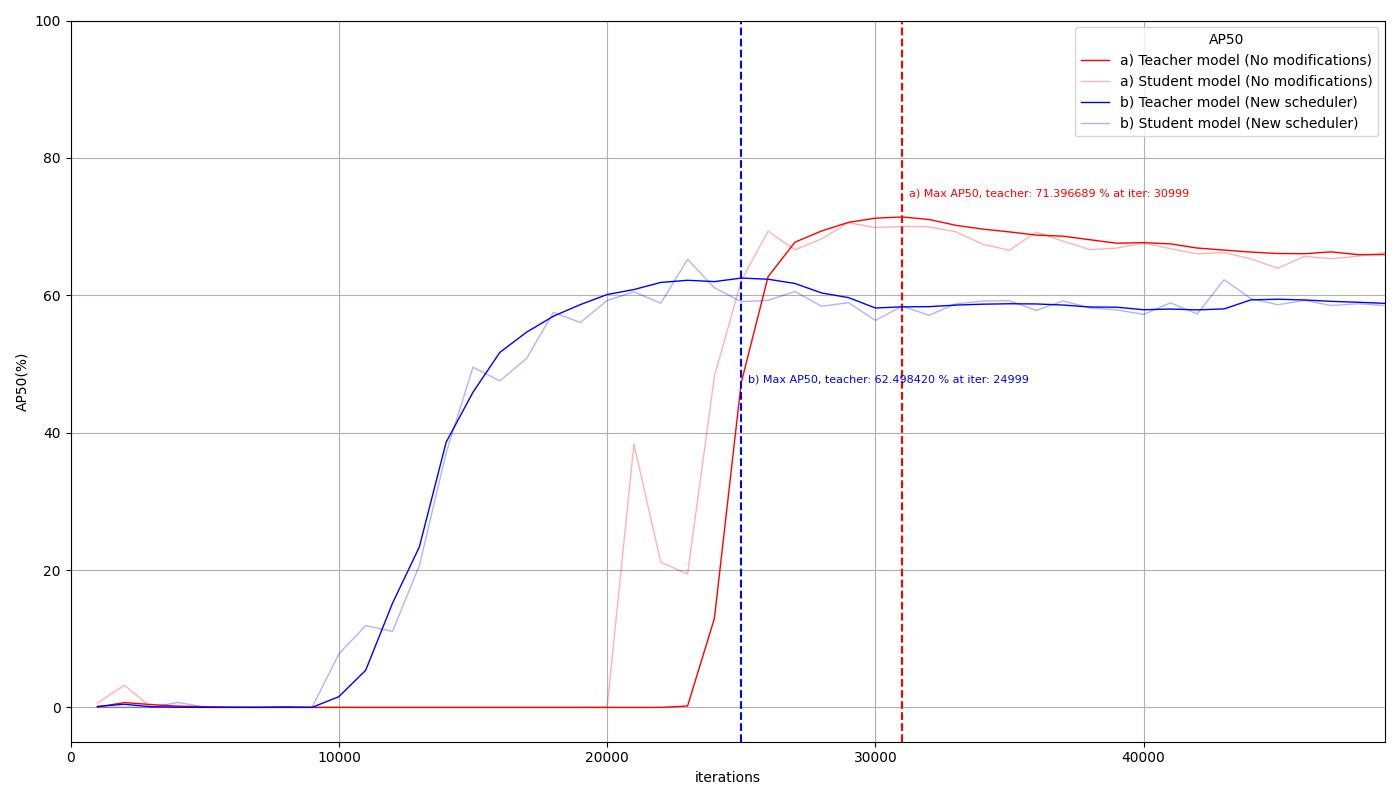
\includegraphics[width=14cm]{./AP50_scheduler.jpg}
	\end{center}
	\caption{a)\texttt{AP50} results of the original model and b) \texttt{AP50} results of the model with a cosine scheduler}
	\begin{center}
		\label{comparison_1}
	\end{center}
\end{figure}
\FloatBarrier

\subsubsection{Additional augmentations}
\label{augmentations_section} 
Following the ideas proposed in Figure \ref{newAugmentations}, an identical model was trained with two additional strong augmentations. Furthermore, in this and the subsequent  experiments, the model leverages the early stopping algorithm with the \texttt{PATIENCE} value of 10. The early stopping algorithm will prevent the model from unnecessary training in case if the AP50 does not improve for more than 10 000 iterations. The results of the evaluation process with the additional augmentations can be found in Figure \ref{augmentation_experiment}. 
 
\begin{figure}[htb]
	\begin{center}
		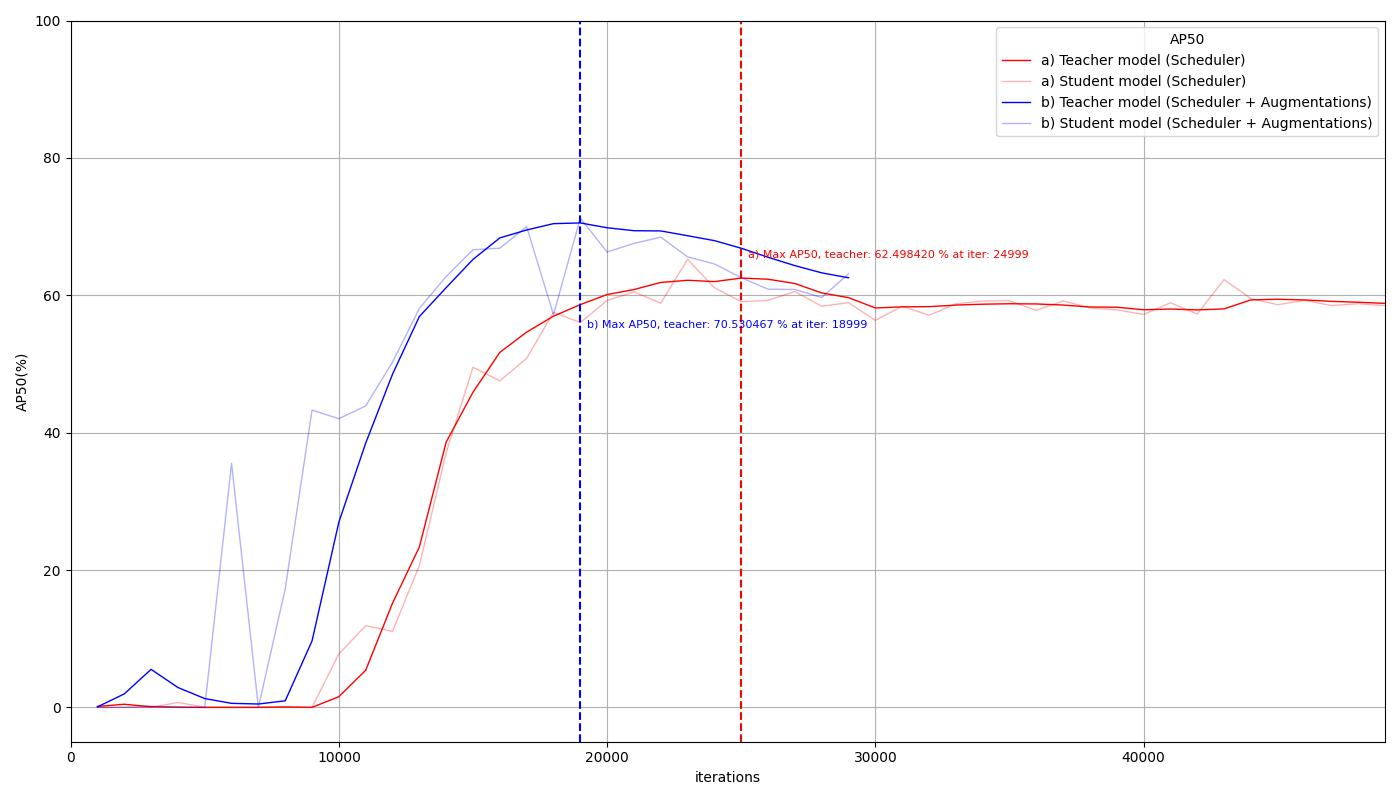
\includegraphics[width=14cm]{./AP50_augmentation.jpg}
	\end{center}
	\caption{a)\texttt{AP50} from the model with a modified scheduler only and b) \texttt{AP50} results of the model with a cosine scheduler and two additional strong augmentations}
	\begin{center}
		\label{augmentation_experiment}
	\end{center}
\end{figure}
\FloatBarrier  

By analyzing these results, it can be easily noticed that the model reaches the peak much faster and the maximum value (\texttt{AP50} = 70.53 \%) is higher than the equivalent model without additional augmentations (\texttt{AP50} = 62.49 \%). Additionally, this model achieves results, which are competitive to the original implementation (71.40 \%).


\subsubsection{Instance-level DA and consistency regularization}
The following set of experiments evaluates the custom model presented in Figure \ref{mymodel}. The model utilizes the same principles as in the previous experiment, which includes the cosine scheduler and additional augmentations. On top of it, in this experiment, an instance-level domain adaptation is added along with the consistency regularization term. The regularization weights from Equation \ref{total_loss} are defined as $\lambda_{\text {consist }} = \lambda_{\text {ins }} = 0.07$. Figure \ref{myModel_experiment} presents the comparison between this model and the model presented in Section \ref{augmentations_section}.

\begin{figure}[htb]
	\begin{center}
		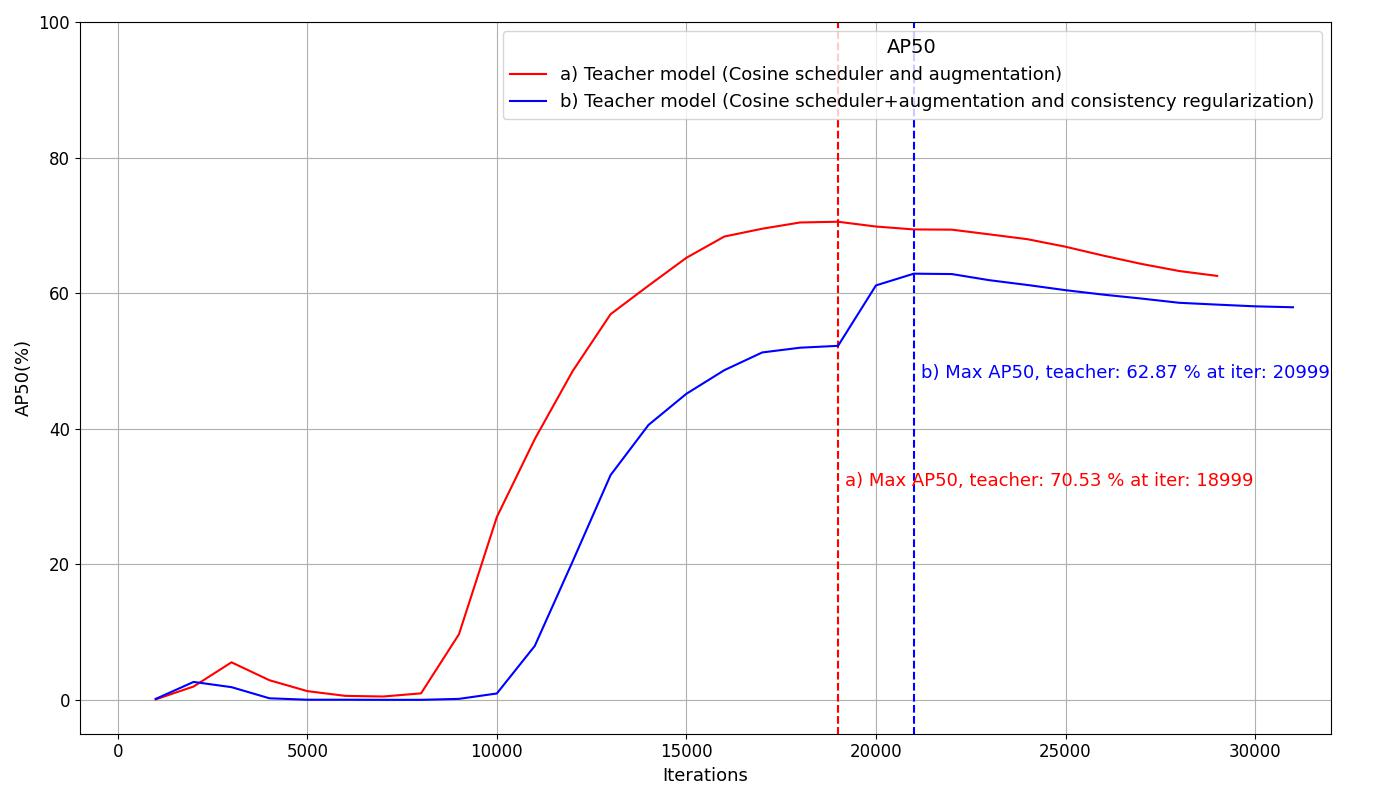
\includegraphics[width=14cm]{./AP50_Augm_consistency.jpg}
	\end{center}
	\caption{a)\texttt{AP50} from the model with a cosine  scheduler and two extra augmentations against b) \texttt{AP50} from the model with a cosine scheduler, two additional augmentations and consistency regularization}
	\begin{center}
		\label{myModel_experiment}
	\end{center}
\end{figure}
\FloatBarrier  

As it can be concluded, the plot with consistency regularization follows a similar pattern as the original model with augmentations. However, the results drop from $max$ (\texttt{AP50}) = 70.53\% back to  $max$ (\texttt{AP50}) = 62.87\%. In order to verify the design of the custom components, an additional experiment was conducted. 

Figure \ref{myModel_constloss_total} illustrates the instance-level loss and consistency loss terms. As it was defined earlier in the \nameref{mainExperiments} section, the model aims to maximize the instance-level alignment loss in order to confuse the classifier and produce domain invariant features. On the other hand, the model also aims to minimize the consistency loss to force both instance- and image-level classifiers to generate identical outputs for the same image. Although both terms are working as designed, as can be concluded from Figure \ref{myModel_constloss_total}, the \texttt{AP50} value does not improve significantly as compared to the original adaptive teacher model. 

\begin{figure}[htb]
	\begin{center}
		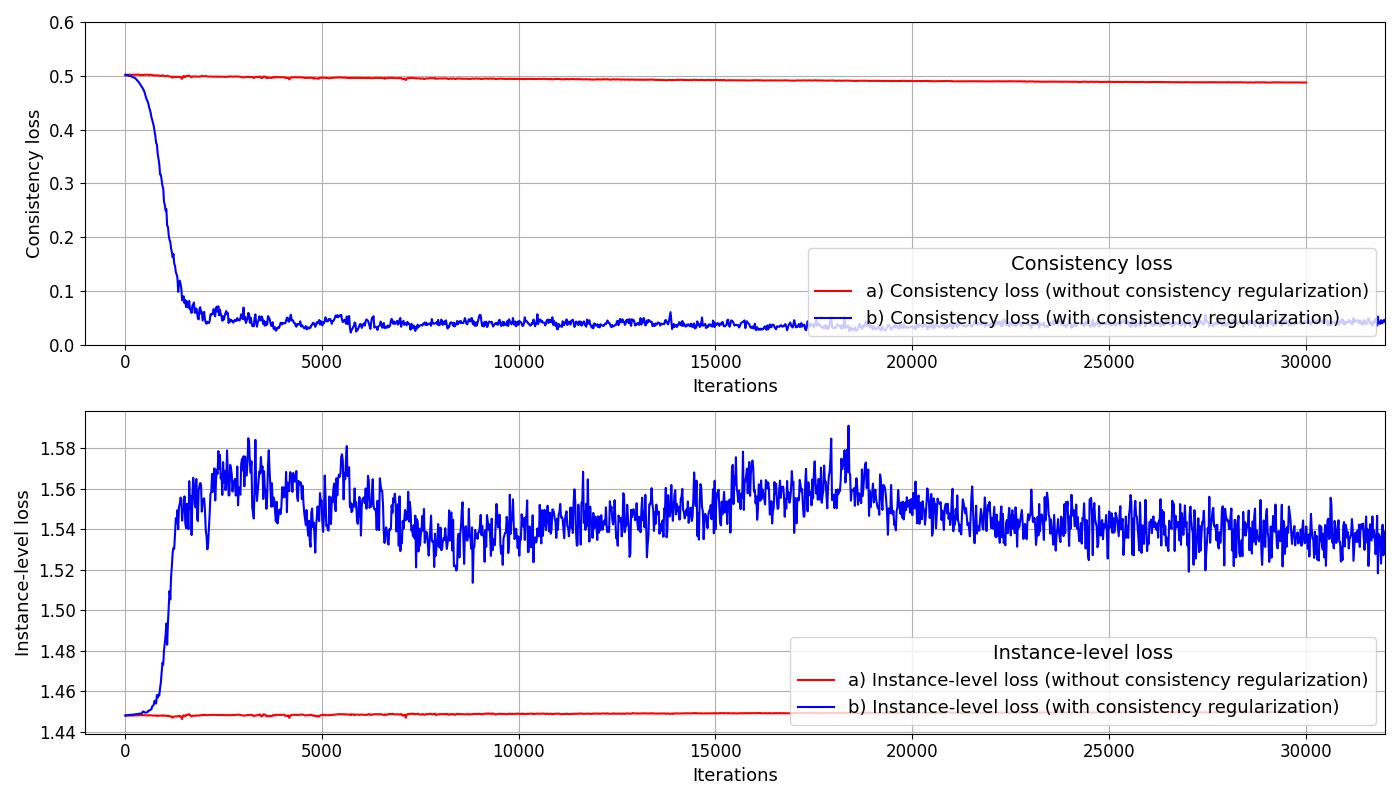
\includegraphics[width=14cm]{./consistency_loss.jpg}
	\end{center}
	\caption{a) The total loss calculation is independent from consistency loss and the instance-level loss terms b) The total loss is proportional to the consistency loss and the instance-level loss terms}
	\begin{center}
		\label{myModel_constloss_total}
	\end{center}
\end{figure}
\FloatBarrier  

A small-scale set of experiments has been additionally carried out in order to identify the optimal weights $\lambda_{\text {consist }}$ and $\lambda_{\text {ins }}$. In order to facilitate the training speed, while preserving fairness in the  comparison, the maximum number of iterations in all experiments was set as \texttt{MAX\textunderscore ITER} = 30 000. Additionally, to decrease the training speed, only the classes 1 to 20 were used for training. The results of six different experiments are shown in Figure \ref{myModel_varying_params}.

\begin{figure}[htb]
	\begin{center}
		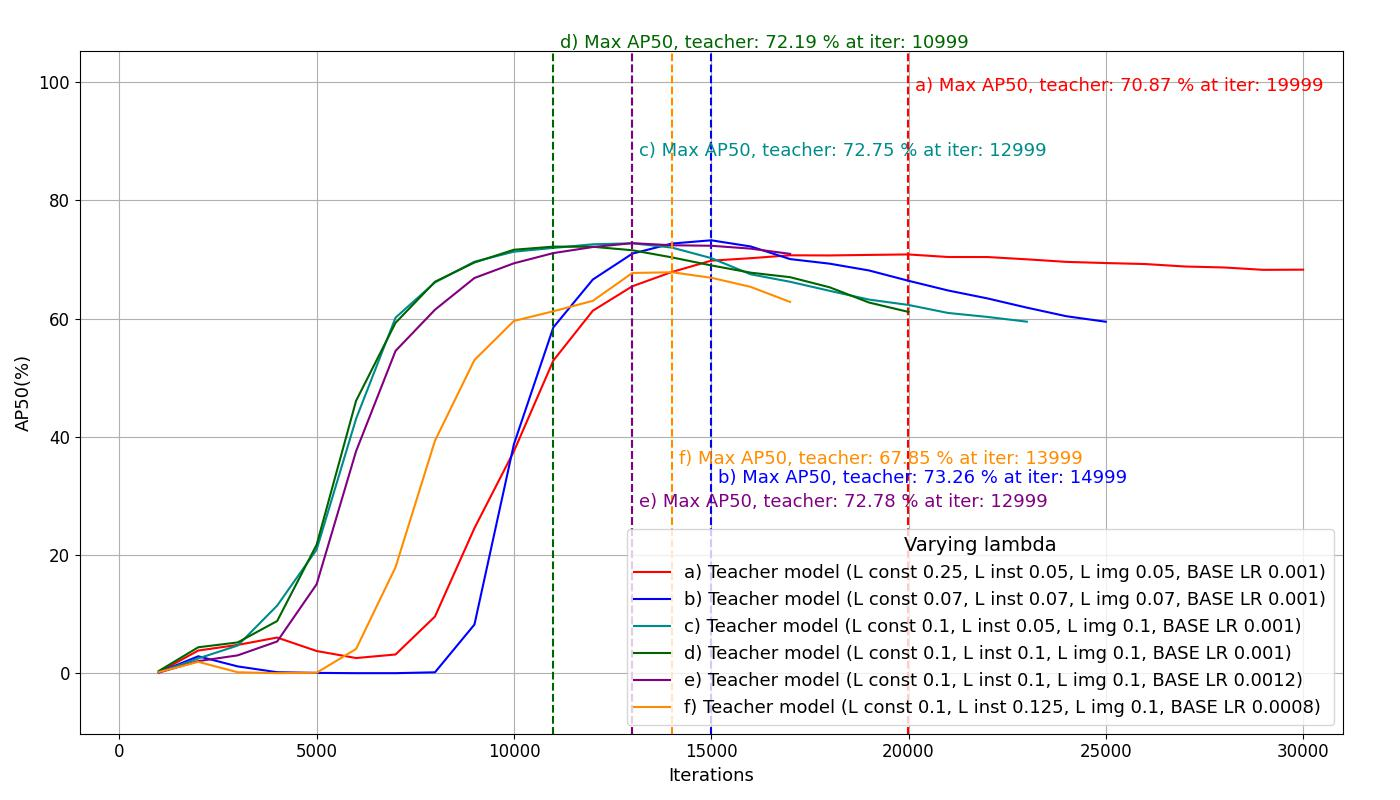
\includegraphics[width=14cm]{./AP50_varying_lambda.jpg}
	\end{center}
	\caption{\texttt{AP50} values for varying weight parameters of $\lambda_{\text {consist }}$, $\lambda_{\text {ins }}$ and \texttt{BASE\textunderscore LR}}
	\begin{center}
		\label{myModel_varying_params}
	\end{center}
\end{figure}
\FloatBarrier  
From these results, the plot with the $\lambda_{\text {consist }} = 0.07$, $\lambda_{\text {ins }} = 0.07$ and \texttt{BASE\textunderscore LR} = 0.001 were identified to be the best parameters with \texttt{AP50} = 73.26 \%. However, in practice, more comprehensive experiments should be carried out to determine the best hyperparameters. 

In order to verify the performance of the components, one last experiment evaluates the network without the cosine scheduler, which seemed to negatively affect the performance of the subsequent experiments the most (see Figure \ref{comparison_1}). The results of the Regularized Cross-Domain Adaptive Teacher model with the original scheduler are presented in Figure \ref{myModel_withOrigSched}.

\begin{figure}[htb]
	\begin{center}
		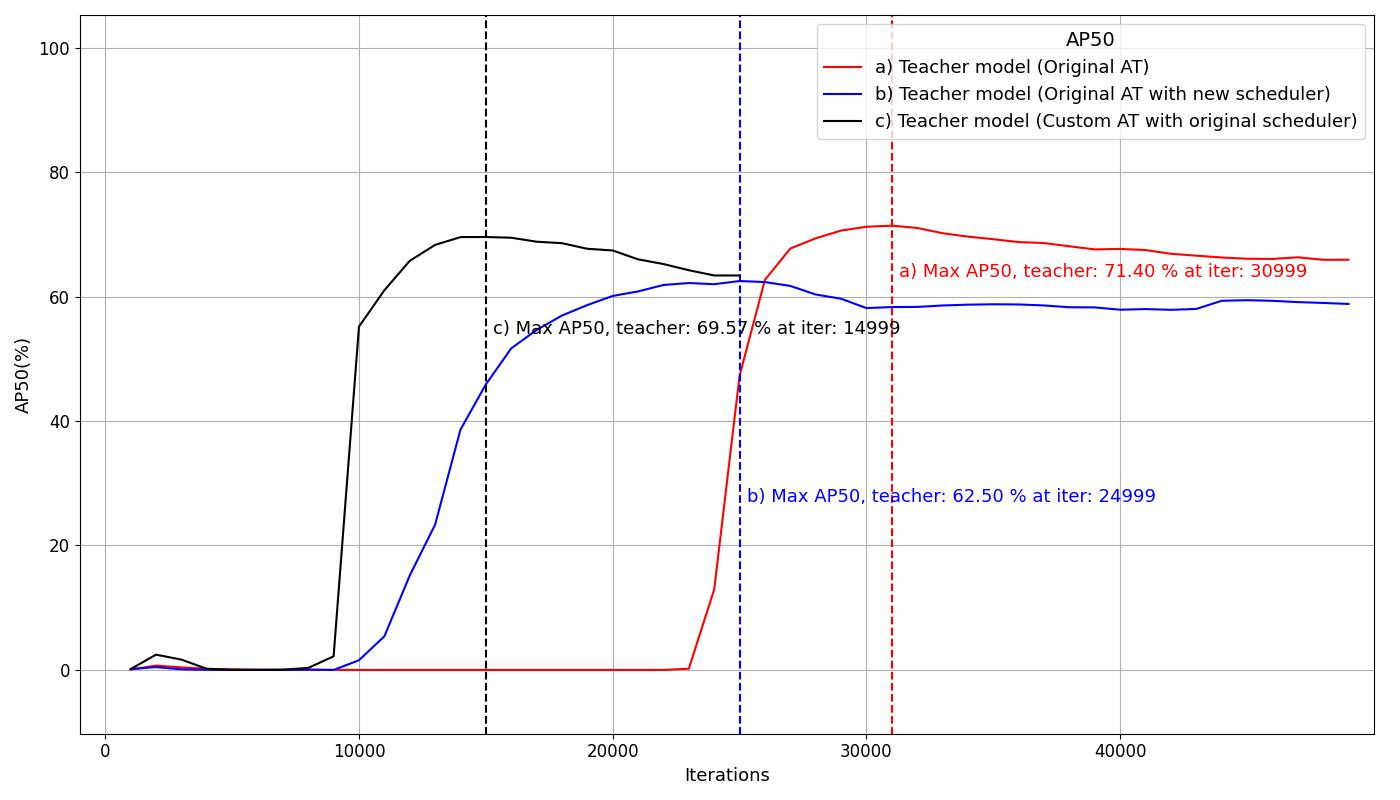
\includegraphics[width=14cm]{./AP50_myModel_origScheduler.jpg}
	\end{center}
	\caption{a) The custom model with the original scheduler b) The custom model with the cosine scheduler c) Original model without any modifications}
	\begin{center}
		\label{myModel_withOrigSched}
	\end{center}
\end{figure}
\FloatBarrier  

According to the results from Figure \ref{myModel_withOrigSched}, the model with regularization and custom augmentation shows competitive results compared to the original Adaptive teacher model with $max$ (\texttt{AP50}) = 69.57\%, while also peaking significantly earlier (>15 000 iterations faster).  

Additionally the obtained results were filtered out and the average of the first four classes \texttt{Model 1..Model 4} were compared to the average of the remaining classes \texttt{Model 5..Model 30}. Essentially, this step has been carried out to verify whether the higher distribution of certain classes affects the model performance (see Figure \ref{tless_distribution_real}). The results can be found in Figure \ref{myModel_withOrigSched_grouped}.     
\begin{figure}[htb]
	\begin{center}
	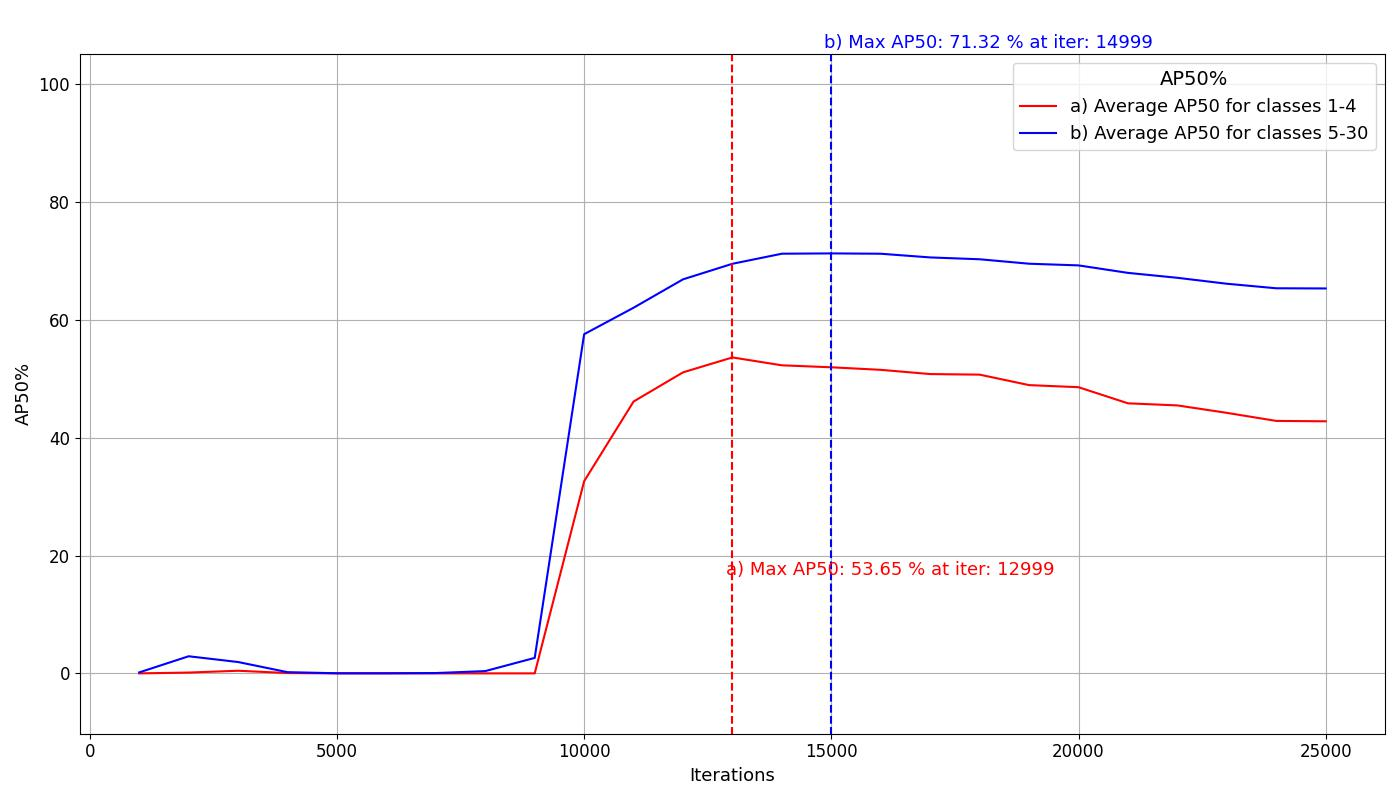
\includegraphics[width=14cm]{./AP50_per_class_group.jpg}
	\end{center}
	\caption{a)\texttt{AP50}}
	\begin{center}
	\label{myModel_withOrigSched_grouped}
	\end{center}
\end{figure}
\FloatBarrier 

\texttt{AP50} = 53.65 \% for the classes \texttt{Model 1..Model 4} seem to be significantly lower than \texttt{AP50} = 71.32 \% for the remaining classes. However, due to a low number of samples, the results might also interpret that the first classes \texttt{Model 1..Model 4} are simply harder to detect. Therefore, more experiments are needed with higher variety in the dataset.  


\subsection{Continual learning results}
\label{cont_learning_results} 
As it was introduced in Figure \ref{tless_distribution_rend}, the entire T-LESS dataset contains 30 different models with objects named arbitrary as \texttt{Model 1..Model 30}. To evaluate the methodology presented in the \nameref{cont_learning_section} section, the following procedure was applied:
 
\begin{enumerate}
\item In the initial experiment, the network was trained on classes \texttt{Model 1..Model 30}.
\item The second network was only trained on the class \texttt{Model 21}.
\item The second network was trained on the classes \texttt{Model 1..Model 20}.
\item The second network was additionally trained to predict the class \texttt{Model 21} in a continuous manner from a pre-trained model that was derived in Step 3.
\end{enumerate} 

\texttt{Model 21} was selected for the first experiment. Ultimately, the performance was evaluated between all four experiments on the single class \texttt{Model 21}. The combined results for a single class are presented in Figure  \ref{myModel_continuous_experiment_1} and the results for the total \texttt{AP50} for the trained dataset are presented in Figure \ref{myModel_continuous_experiment_3}.

\begin{figure}[htb]
	\begin{center}
		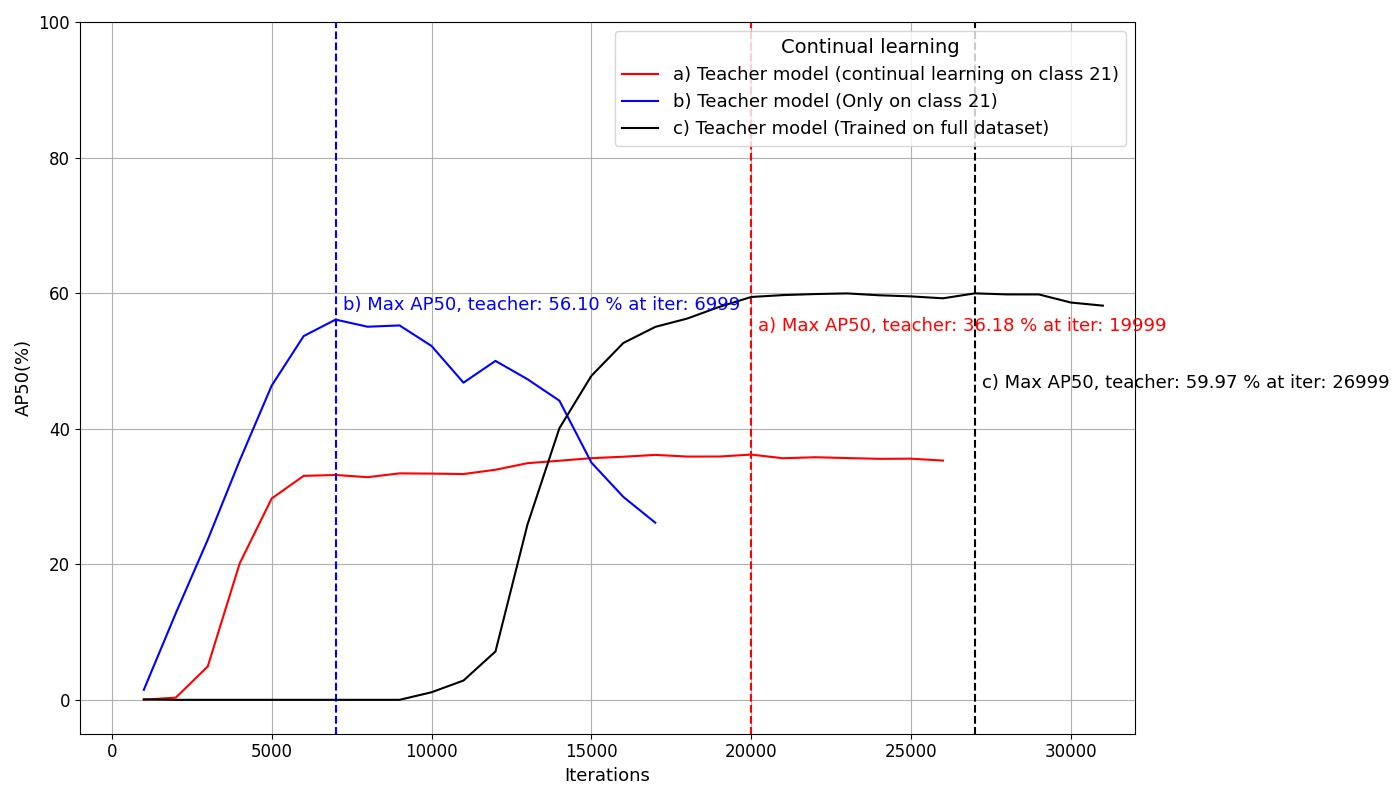
\includegraphics[width=14cm]{./AP50_continual_21.jpg}
	\end{center}
	\caption{The \texttt{AP50} results for class \texttt{Model 21} evaluated on different networks}
	\begin{center}
		\label{myModel_continuous_experiment_1}
	\end{center}
\end{figure}
\FloatBarrier  

\todo{check this} 
\begin{figure}[htb]
	\begin{center}
		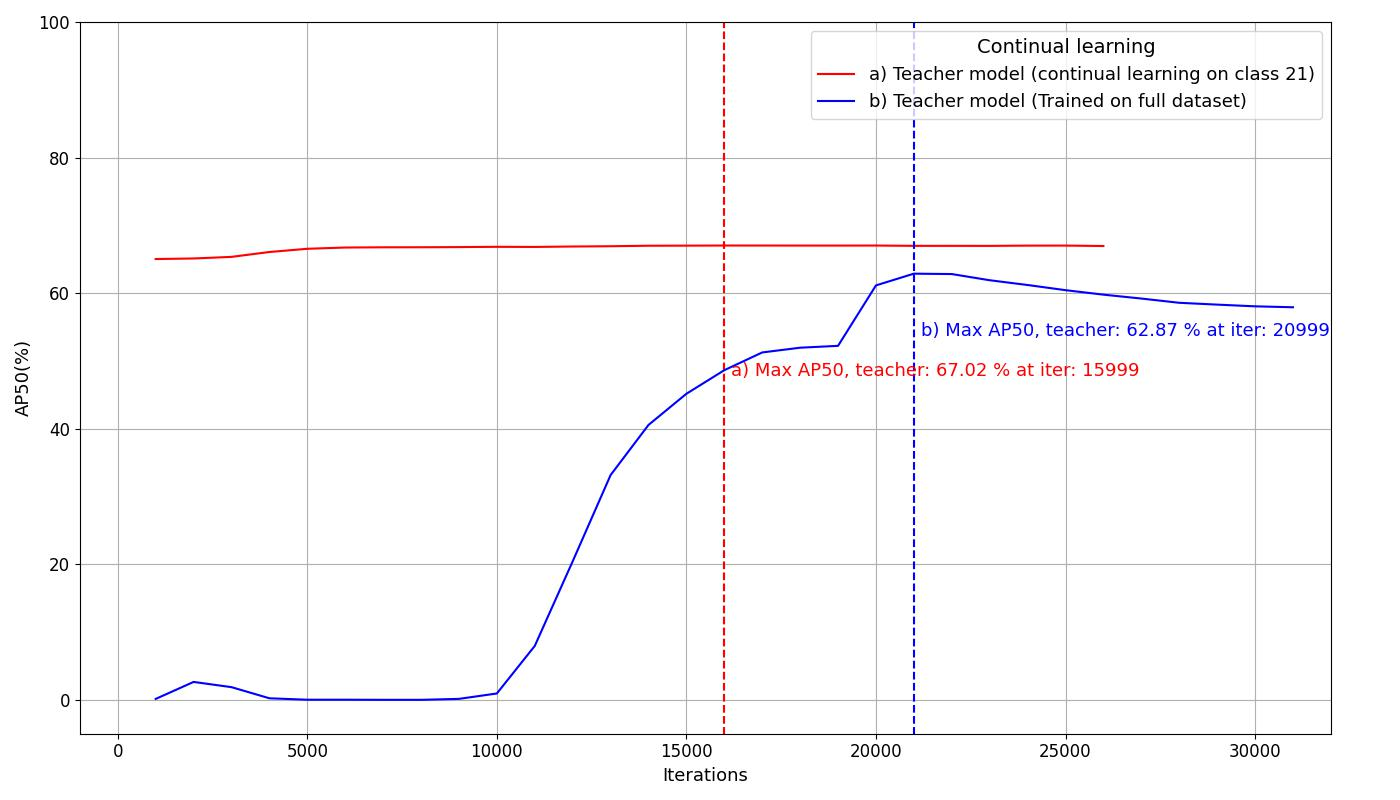
\includegraphics[width=14cm]{./AP50_continual_21_allClasses.jpg}
	\end{center}
	\caption{a)The total continual \texttt{AP50} results evaluated on the classes (\texttt{Model 1..Model 21}) b) The total \texttt{AP50} results for the }
	\begin{center}
	\label{myModel_continuous_experiment_3}
	\end{center}
\end{figure}
\FloatBarrier 

The model trained purely on the \texttt{Model 21} (Figure \ref{myModel_continuous_experiment_3} (a))  rises just as rapidly as it declines. This is contrary to the model trained on the entire dataset (Figure \ref{myModel_continuous_experiment_3} (b)), which takes longer to train but also grants better performance on the given class. On the other hand, the model trained in a continual manner (Figure \ref{myModel_continuous_experiment_3} (c)) learns the new class almost just as fast as the model trained purely on the \texttt{Model 21}. However, after a while it stagnates and barely reaches 36\%. Similar pattern repeats for other classes of objects when Steps 2 and 4 are repeated, as can be found in Figure \ref{myModel_continuous_experiment_2}.

\begin{figure}[htb]
	\begin{center}
		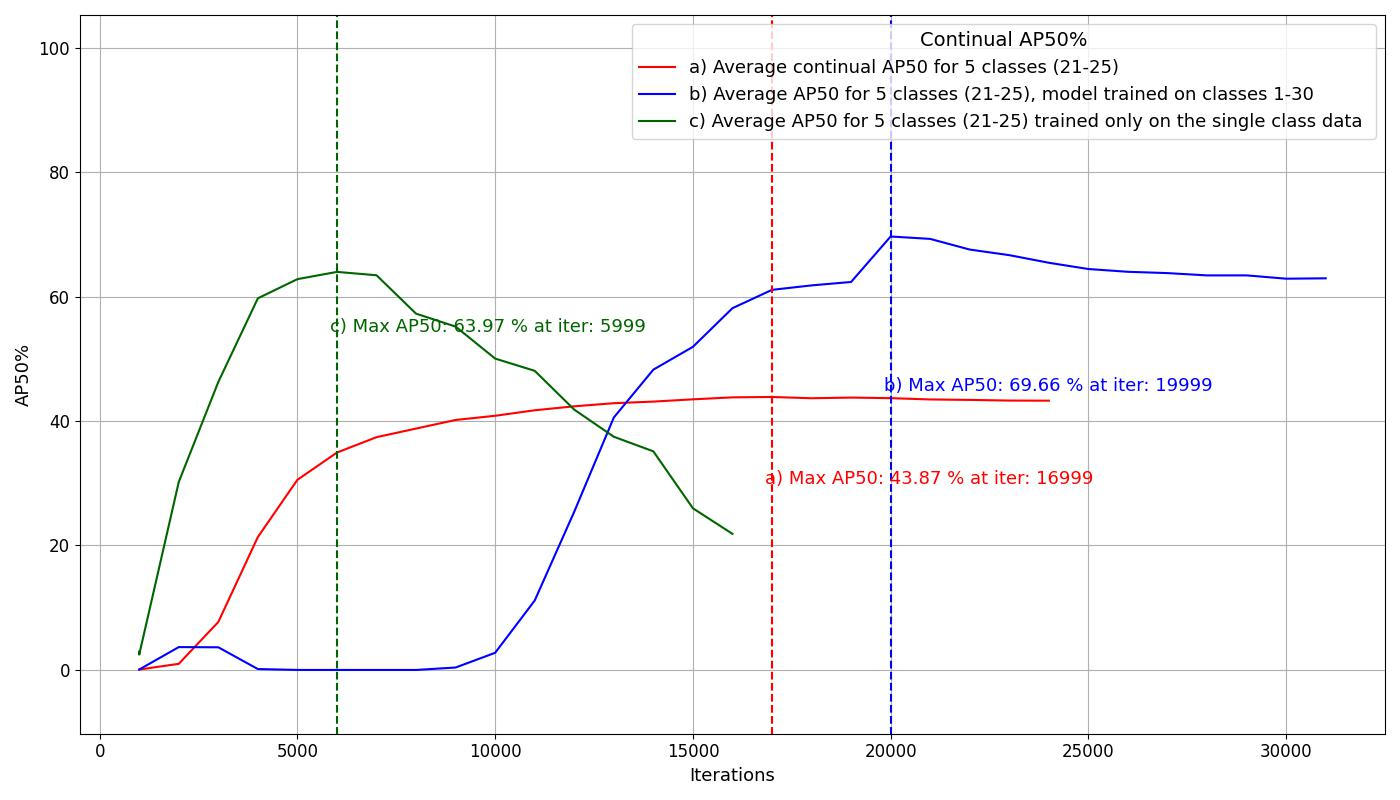
\includegraphics[width=14cm]{./continualAP_average.jpg}
	\end{center}
	\caption{a)The average \texttt{AP50} value for continual learning on classes \texttt{Model 21..Model 25} given the model trained on classes \texttt{Model 1..Model 20}  b)The average \texttt{AP50} value for classes \texttt{Model 21..Model 25} extracted from the regular model trained on classes \texttt{Model 1..Model 30} c) The \texttt{AP50} value for each of the classes \texttt{Model 21..Model 25} when trained only on its own. The values are then averaged out for all 5 classes }
	\begin{center}	\label{myModel_continuous_experiment_2}
	\end{center}
\end{figure}
\FloatBarrier
  
Here,  the Steps 2 and 4 were repeated for the classes \texttt{Model 21..Model 25}. Consequently, the average of these results for each class were combined to form the plot in Figure \ref{myModel_continuous_experiment_2} (a). On the other hand, the results of the training on the entire dataset were extracted and the plot in  \ref{myModel_continuous_experiment_2} was generated, which includes the average results between the same classes \texttt{Model 21..Model 25}. Finally, Figure \ref{myModel_continuous_experiment_2} (c) illustrates the \texttt{AP50} value for the average of each of the classes \texttt{Model 21..Model 25} when trained separately. As it can be concluded, training the model with more classes improves the quality of the detection from 63.97 \% to 69.66 \%. Additionally, it can be noted that the model trains significantly better when trained from the scratch \texttt{AP50} = 69.66\%, compared to the model trained continuously (\texttt{AP50} = 43.87\%). However, it takes considerably less time to train the model continuously.

Although the method seems to fail in learning a new class efficiently, it has proven to hold well against the catastrophic forgetting problem discussed in Section \ref{cont_learning}, as discussed in Figure \ref{myModel_continuous_experiment_3}. 

\subsection{Deployment results}
In order to showcase the performance, a simple web app was prepared. The app was hosted on a local server and it leverages Flask API to attach the detector app to a user interface. The app utilizes the model, which was presented in Figure \ref{myModel_withOrigSched} due to its relatively good performance and the fastest training speed. The prototype of the UI is presented in Figure \ref{demo}. 

\todo{update the picture} 
\begin{figure}[htb]
	\begin{center}
		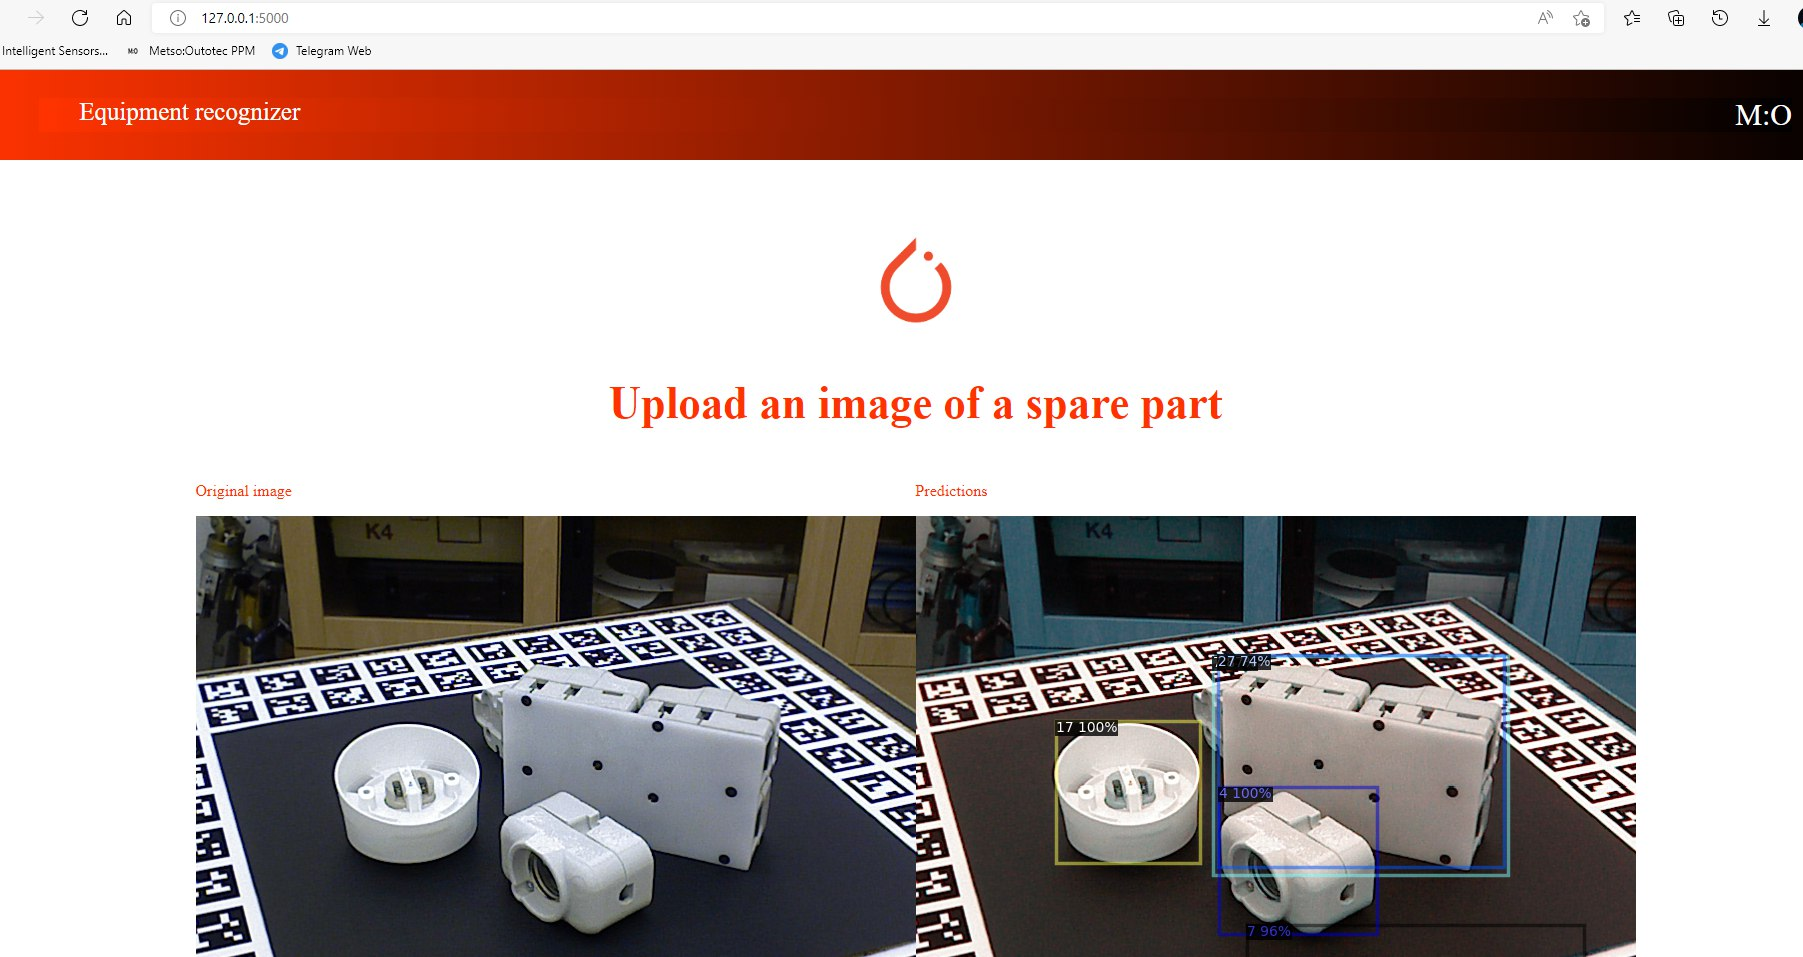
\includegraphics[width=14cm]{./demo.png}
	\end{center}
	\caption{A screenshot of the simple web app. The image on the left-hand side is an uploaded target image, and the image on the right-hand side shows a prediction of the objects.}
	\begin{center}
		\label{demo}
	\end{center}
\end{figure}

The app sends \texttt{POST} requests to upload an image to localhost via Flask API. The image is then processed in the model and returned to the user interface. The complete app runs on Python 3.9, while the model additionally utilizes packages and frameworks such as Pytorch 1.10.1, CUDA 11.3 and Detectron2 v0.6. For model training, Nvidia A100 GPU units were used. The hardware and the computing resources were provided by CSC - Finnish IT Center for Science. For model interference, a standard CPU node was used. 

\clearpage